\section{Neural Fourier Filter Banks}
\par 
    Στο πεδίο της \enit{3D} όρασης, (De Queiroz κ.α. \cite{de2016compression}) πρότειναν την χρήση προσαρμοστικής περιοχής του ιεραρχικού χωρικού μετασχηματισμού κυματιδίων (\enit{Adaptive region Hoar Wavelets}) για την διευκόλυνση συμπίεσης νέφους σημείων \enit{3D}. Συγχρόνως οι Ιsik, κ.α. \cite{isik2022lvac} προτείνουν την εκμάθηση των ογκομετρικών χαρακτηριστικών που προκύπτουν από την προηγούμενη εργασία από δίκτυα συντεταγμένων. Τέλος δίνεται μια προοπτική στην ανακατασκευή αναπαραστάσεων με φίλτρα κυματιδίων(\enit{wavelet filtering}), για συμπαγή πεδία νευρικής ακτινοβολίας στην εργασία \cite{Rho_2023_CVPR}.

\par
    Πριν λίγους μήνες από το εργαστήριο \enit{UBC-Vision(University of British Columbia Computer Vision Group)} δημοσιεύτηκε ένα κείμενο που προτείνει έναν συνδυασμό των παραπάνω μεθόδων κωδικοποίησης που μπορεί να εφαρμοστεί και σε δεδομένα εικόνας αλλά σημαντικό είναι πως μπορεί να εφαρμοστεί και σε δεδομένα που αναπαριστούν έμμεσα πεδία γεωμετρίας. 
\par 
    Ο λόγος γίνεται για την έρευνα \enit{Neural Fourier Filter Banks} \cite{wu2023neural}, η οποία βασιζόμενη στην ιδέα συχνοτικής αποσύνθεσης του σήματος με χρήση κυματιδίων (\enit{Wavelet Decomposition}), προτείνει την επικουρική χρήση και των δικτύων που εφαρμόζουν κωδικοποίηση της εισόδου με χρήση εφαπτόμενου πυρήνα Fourier, και των δικτύων που εφαρμόζουν χωρική κωδικοποίηση συντεταγμένων με έ´ναν τρόπο που διατηρούνται τα χαρακτηριστικά και των δύο μορφών κωδικοποίησης.
\par
    Η αρχιτεκτονική του δικτύου που προτείνεται φαίνεται στην παρακάτω εικόνα και στην παρούσα εργασία με βάση την παρακάτω εικόνα προσπαθεί να επινοηθεί μια μέθοδος που εφαρμόζει αυτή την διαδικασία στα δεδομένα στοχεύοντας αποτελέσματα υψηλής αξιοπιστίας ανακατασκευής σε μικρότερο αριθμό εποχών εκπαίδευσης του δικτύου απόδοσης IDR \cite{yariv2020multiview}.
\begin{figure}[H]
    \centering
    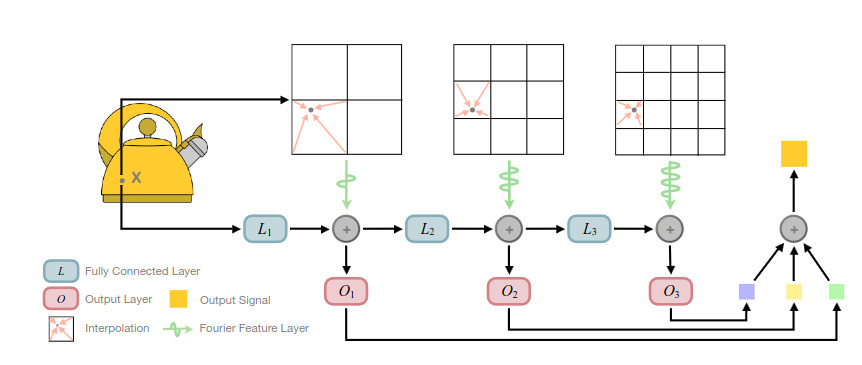
\includegraphics[width=.57\linewidth]{images/chapter3_img/nffb_og_architecture.jpg}
    \caption{Προτεινόμενη αρχιτεκτονική NFFB, Πηγή \cite{wu2023neural}}
    \label{fig:nffbogarchitecture}
\end{figure}
\clearpage